\documentclass[11pt]{amsart}

\usepackage[usenames,dvipsnames,svgnames,table]{xcolor}
\usepackage[colorlinks=true, pdfstartview=FitV, linkcolor=blue, citecolor=blue, urlcolor=blue]{hyperref}

\usepackage[centering]{geometry}                % See geometry.pdf to learn the layout options. There are lots.
\geometry{letterpaper}                   % ... or a4paper or a5paper or ...
%\geometry{landscape}                % Activate for for rotated page geometry
%\usepackage[parfill]{parskip}    % Activate to begin paragraphs with an empty line rather than an indent
\usepackage{graphicx}
\usepackage{amssymb}
\usepackage{epstopdf}
\usepackage{lscape}
\usepackage{xcolor}
\usepackage[utf8]{inputenc}
\usepackage{tikz,caption}
\DeclareGraphicsRule{.tif}{png}{.png}{`convert #1 `dirname #1`/`basename #1 .tif`.png}
\usepackage{enumitem}
\setlist[itemize]{leftmargin=2em}
\setlist[enumerate]{leftmargin=2em}
\usepackage{booktabs}
\usepackage{multirow}
\usepackage{mathtools}
\usepackage{mathrsfs}
\usepackage[aligntableaux=center, smalltableaux]{ytableau}
\usepackage{youngtab}
\usepackage{verbatim}
\usepackage{faktor}

\usepackage{stmaryrd}

\newtheorem{thm}{Theorem}

\definecolor{darkblue}{rgb}{0.0,0,0.7} % darkblue color
\definecolor{darkred}{rgb}{0.7,0,0} % darkred color
\definecolor{darkgreen}{rgb}{0, .6, 0} % darkgreen color

% Dark red emphasis
\newcommand{\defncolor}{\color{darkred}}
\newcommand{\defn}[1]{{\defncolor\emph{#1}}} % emphasis of a definition

\newtheorem{theorem}{Theorem}[section]
\newtheorem{proposition}[theorem]{Proposition}
\newtheorem{property}[theorem]{Property}
\newtheorem{corollary}[theorem]{Corollary}
\newtheorem{question}[theorem]{Question}
\newtheorem{lemma}[theorem]{Lemma}
\newtheorem{conjecture}[theorem]{Conjecture}
\theoremstyle{definition}
\newtheorem{definition}[theorem]{Definition}
\newtheorem{example}[theorem]{Example}
\newtheorem{remark}[theorem]{Remark}
\numberwithin{equation}{section}

\def\NN{{\mathbb N}}
\def\CC{{\mathbb C}}
\def\ZZ{{\mathbb Z}}

\DeclareMathOperator{\GL}{GL}
\DeclareMathOperator{\OPG}{OPG}

\usepackage[colorinlistoftodos]{todonotes}

\newcommand{\mike}[1]{\todo[size=\tiny,color=green!30]{#1 \\ \hfill --- Mike}}
\newcommand{\lucas}[1]{\todo[size=\tiny,color=red!50]{#1 \\ \hfill --- Lucas}}
\newcommand{\felix}[1]{\todo[size=\tiny,color=Cyan]{#1 \\ \hfill --- Félix}}
\newcommand{\farhad}[1]{\todo[size=\tiny,color=blue!50]{#1 \\ \hfill --- Farhad}}
\newcommand{\eric}[1]{\todo[size=\tiny,color=BurntOrange!50]{#1 \\ \hfill --- Eric}}
\newcommand{\nicolas}[1]{\todo[size=\tiny,color=purple!50]{#1 \\ \hfill --- Nicolas}}
\setlength{\marginparwidth}{28mm}

\title{Catalan Hopf sub-algebras of $\mathsf{NCSym}$}
\author{}

\begin{document}
\maketitle

\section{Project description}

\noindent
To identify all the Hopf sub-algebras of $\mathsf{NCSym}$ that are of dimension Catalan and classify them.


\begin{itemize}
\item Introduction - notation and background
\cite{AT20, BBT14, BHRZ05, B08, BZ09, F12, LM11, NT05, RS06}
\cite{S09}
\begin{itemize}
\item Set partitions, non-crossing and non-nesting
\item $\mathsf{NCSym}$ as a Hopf algebra of set partitions which is non-commutative but co-commutative.
\item (Relevant/useful) bases and known formulae for the product and coproduct.
\item subalgebras characterized by primitives
\end{itemize}
\item I think that we have identified all of the possible Hopf subalgebras of $\mathsf{NCSym}$
(or at least the ones that are characterized by their basis of primitives, which I think is all of them).
Let $b_i$ be the number of atomic set partitions of size $i$, for each sequence of integers $(\mathbf{a}) = (a_1, a_2, a_3,\ldots)$ such that
$0 \leq a_i \leq b_i$ there is a Hopf subalgebra $H^{(\mathbf{a})}$.
Let $H^{(\mathbf{a})}_n$ be the graded component of degree $n$,
$$\mathrm{dim}~H^{(\mathbf{a})}_n = \hbox{coefficient of }t^n\hbox{ in }\frac{1}{1 - a_1 t - a_2 t^2 - a_3 t^3 - \cdots}~.$$
\end{itemize}

\section{Notation}

A \defn{composition} of $n$ is a sequence $\beta = (\beta_1, \beta_2, \ldots, \beta_\ell)$ of positive integers such that $\beta_{1} + \beta_{2} + \cdots + \beta_{\ell} = n$.  
We refer the the integers $\beta_{i}$ as the parts of $\beta$ and write $\ell(\beta)$ for the length of $\beta$, which is the number of parts.  
We will use the notation $\beta \vDash n$ to indicate that $\beta$ is a composition of $n$.

We say that $\lambda$ is a \defn{partition} of $n$, if $\lambda \vDash n$ and
$\lambda_1 \geq \lambda_2 \geq \cdots \geq \lambda_{\ell(\lambda)}$.  We will indicate that $\lambda$ is a partition
of $n$ with the notation $\lambda \vdash n$.  We will also use the notation $m_d(\lambda)$ to be the number of times
that $d$ appears as a part in $\lambda$.

Let $\CC^{\NN}$ denote the space of infinite sequences $(c_{n})_{n \ge 1} = (c_{1}, c_{2}, \ldots)$ of complex numbers, i.e.~$c_{n} \in \CC$ for all $n \ge 1$.  
Given two sequences $\vec{c} = (c_{1}, c_{2}, \ldots)$ and $\vec{d} = (d_{1}, d_{2}, \ldots)$, we write
\[
\vec{c} \le \vec{d} 
\qquad\text{if and only if}\qquad
\text{$c_{n} \le d_{n}$ for all $n \ge 1$}.
\]
Let $\vec{0} \in \CC^{\NN}$ denote the zero sequence, so that $\vec{c} \ge \vec{0}$ is and only if $\vec{c}$ consists of entirely nonnegative entries.  
For a composition $\alpha = (\alpha_{1}, \alpha_{2}, \ldots, \alpha_{\ell}) \vDash n$, define 
\[
c_{\alpha} = c_{\alpha_{1}} c_{\alpha_{2}} \cdots c_{\alpha_{\ell}}.
\]
Note that $c_{\alpha} = c_{\beta}$ whenever $\beta \vDash n$ is a composition with the same parts as $\alpha$ in a possibly different order, i.e.~ $\beta_{i} = \alpha_{\sigma(i)}$ for some permutation $\sigma$ of the integers $\{1,2, \ldots, \ell(\alpha)\}$.


Given a sequence $\vec{a}$ consisting of nonnegative integers, let 
\[
X(\vec{a}) = \biguplus_{n \ge 1} \{x^{(n)}_{i} \;|\; 1 \le i \le a_{n} \}.
\]
and let $\mathfrak{L}(\vec{a})$ denote the free graded Lie algebra on the graded set $X(\vec{a})$.  

For a graded Lie algebra $L$, $\mathcal{U}(L)$ will denote the universal enveloping (Hopf) algebra of $L$.  
For a graded Hopf algebra $H$, $\mathcal{P}(H)$ will denote graded Lie algebra of primitives, so that
\[
\mathcal{P}(H) = \{x \in H \;|\; \Delta(x) = 1 \otimes x + x \otimes 1\}.
\]

\section{Combinatorics of sequences of numbers}

Our main results make use of three interrelated sequences that we will denote by $\vec{h}$, $\vec{a}$, and $\vec{p}$.  
In this section we take a purely enumerative perspective to these sequences, assuming only that they satisfy the relation given in Equation~\eqref{eq:gf_relation}.
However, in later sections these sequences come from a combinatorial Hopf algebra $H$, which will provide useful motivation here:
\begin{itemize}
\item $\vec{h} = (h_{1}, h_{2}, \ldots)$ will be the graded dimensions of $H$,

\item $\vec{a} = (a_{1}, a_{2}, \ldots)$ will be the graded numbers of free generators of the algebra, and 

\item $\vec{p} = (p_{1}, p_{2}, \ldots)$ will be the graded dimension of the Lie algebra of primitives $\mathcal{P}(H)$.

\end{itemize}

To define our sequences, we make use of the fact---recorded in Proposition~\ref{prop:sequences} below---that any formal power series in $\CC[[t]]$ with constant term $1$ can be expressed in three equivalent ways,
\begin{equation}
\label{eq:gf_relation}
1 + \sum_{k \geq 1} h_k t^k = \frac{1}{1 - \sum_{m \geq 1} a_m t^m} = \prod_{d \geq 1} \frac{1}{(1-t^d)^{p_d}}~.
\end{equation}
which determines a triple of sequences: $(\vec{h}, \vec{a}, \vec{p})$ with $\vec{h} = (h_{1}, h_{2}, \ldots)$, $\vec{a} = (a_{1}, a_{2}, \ldots)$, and $\vec{p} = (p_{1}, p_{2}, \ldots)$.  

\begin{example}
Take $f(t) = 1 + 2t + 3 t^{2} + \cdots \in \CC[[t]]$, so that $\vec{h} = (1, 2, 3, \ldots)$.  Then $f(t)$ is a geometric series,
\[
f(t) = \frac{1}{1 - 2 t^{2} + t^{2}} = \frac{1}{(1-t)^{2}}
\]
so the remaining sequences are $\vec{a} = (2, -1, 0, \ldots)$ and $\vec{p} = (2, 0, 0, \ldots)$.
\lucas{This is a boring example, but I am putting it in as a placeholder.}
\end{example}

We will make extensive use of explicit formulas relating the sequences $\vec{h}$, $\vec{p}$, and $\vec{a}$.  While these are well-known, we include a proof for the sake of completeness.

\begin{proposition}
\label{prop:sequences}
Any one sequence $\vec{h}$, $\vec{a}$, or $\vec{p} \in \CC^{\NN}$ belongs to a unique triple $(\vec{h}, \vec{a}, \vec{p})$ of sequences that satisfy Equation~\eqref{eq:gf_relation}, given by:
\begin{enumerate}[label = (\roman*), itemsep = 1em]
\item $\displaystyle h_{n}
= \sum_{\beta \vDash n} a_\beta
= \sum_{\lambda \vdash n} \prod_{d \geq 1} \binom{p_d + m_d(\lambda) -1}{p_d -1}$, 

\item $\displaystyle a_n
= \sum_{\beta \vDash n} (-1)^{\ell(\beta)-1} h_\beta
= \sum_{\lambda \vdash n} (-1)^{\ell(\lambda)-1} \prod_{d \geq 1} \binom{p_d}{m_d(\lambda)}$, and

\item $\displaystyle p_n
= \sum_{d|n} \sum_{\beta \vDash d} \frac{d\cdot \mu(n/d)}{n \cdot \ell(\beta)} a_\beta
= \sum_{d|n} \sum_{\beta \vDash d} \frac{d\cdot \mu(n/d) (-1)^{\ell(\beta)-1}}{n \cdot \ell(\beta)} h_\beta$.

\end{enumerate}
\end{proposition}

\begin{proof}
%We will make use of the identities
%\[
%(1-t)^p = \sum_{k \geq 0} \binom{p}{k} t^k, \quad
%\frac{1}{(1-t)^p} = \sum_{k \geq 0} \binom{p+k-1}{p-1} t^k, \quad\text{and}\quad
%\log(1-t) = \sum_{j \geq 1} \frac{t^j}{j}
%\]
%to derive equations (i)--(iii) from Equation \eqref{eq:gf_relation}.

In order to see (i), take the geometric series expansion of the second and third expressions in Equation \eqref{eq:gf_relation} to obtain
\begin{equation}\label{eq:gf_relation}
1 + \sum_{k \geq 1} h_k t^k = \sum_{k \geq 0} \left(\sum_{m \geq 1} a_m t^m\right)^k = \prod_{d \geq 1}
\left(\sum_{k \geq 0} \binom{p_d+k-1}{p_d-1} t^{kd}\right).
\end{equation}
Expanding each product of sums and isolating the coefficient of $t^{n}$ in each expression gives the desired equation.

Now we prove (ii).  Take the reciprocal of Equation \eqref{eq:gf_relation} to obtain
\[
1 - \frac{1}{1 + \sum_{k \geq 1} h_k t^k} 
= \sum_{m \geq 1} a_m t^m 
= \prod_{d \geq 1} (1-t^d)^{p_d}.
\]
Expanding the left- and rightmost expressions yields
\[
\sum_{r \geq 1} (-1)^{r-1} \left(\sum_{k \geq 1} h_k t^k\right)^r
= \sum_{m \geq 1} a_m t^m
= \prod_{d \geq 1} \sum_{k \geq 0} \binom{p_d}{k} t^{dk}.
\]
Isolating the coefficient of $t^{n}$, we obtain equation (ii).

Finally, we deduce (iii).  Beginning with the reciprocal of Equation \eqref{eq:gf_relation} as above, take the logarithm of each term and Taylor expand about $1$ to obtain
%
%giving
%\[
%-\log\left( 1 + \sum_{k \geq 1} h_k t^k \right)
%= \log\left( 1 - \sum_{m \geq 1} a_m t^m \right)
%= \sum_{d \geq 1} p_d \log( 1-t^d ).
%\]
%Replacing each logarithm with its Taylor expansion about $1$, this becomes
\[
 \sum_{r \geq 1} \frac{(-1)^{r-1}(\sum_{k \geq 1} h_k t^k )^r}{r}
= \sum_{r \geq 1} \frac{(\sum_{m \geq 1} a_m t^m )^r}{r}
= \sum_{d \geq 1} \sum_{j \geq 1} p_d \frac{t^{jd}}{j}.
\]
Now we isolate the coefficient of $t^{n}$ in each of the expressions: 
\[
\sum_{\beta \vDash n} \frac{a_\beta}{\ell(\beta)}
= \sum_{\beta \vDash n} \frac{(-1)^{\ell(\beta)-1} h_\beta}{\ell(\beta)}
= \frac{1}{n} \sum_{d | n} d p_{d} .
\]
Lastly, multiply the equation by $n$ and apply M\"{o}bius inversion to solve for $p_{d}$.
\end{proof}


If the sequence $\vec{a}$ consists of entirely non-negative integers, $\vec{h}$ and $\vec{p}$ also have combinatorial interpretation in terms of words.
Recall that a word in a set $X$ is a finite sequence $w = w_{1} w_{2} \ldots w_{\ell}$ of ``letters'' $w_{i} \in X$.  
If $X = \bigcup_{n \geq 1} X^{(n)}$ is a graded set, then define the \emph{degree} of a word to be
%$x \in X^{(n)}$ to be $n$, and let
\[
\mathsf{deg}(w_1 w_2 \ldots w_{\ell}) = \sum_{i = 1}^{\ell} \mathsf{deg}(w_{i})
\qquad\text{where $\mathsf{deg}(x) = n$ for all $x \in X^{(n)}$}.
%\qquad\text{for $d_{i}$ such that $w_{i} \in X^{(d_{i})}$}.
\]
For a fixed order on $X$, we order the words on $X$ lexicographically.  
The \emph{rotation} of a word $w = w_{1} w_{2} \ldots w_{\ell}$ is the word
\[
\mathsf{cyc}(w) =  w_{2} \ldots w_{\ell} w_{1}.
\]
This defines an operation of order $\ell$ on words of with $\ell$ letters.  
A word is \emph{Lyndon} if it is strictly smaller than each of $\mathsf{cyc}(w), \mathsf{cyc}^{2}(w), \ldots, \mathsf{cyc}^{\ell-1}(w)$.  
For instance, if $X = \{x < y\}$, then $xyxyy$ is a Lyndon word, but neither $xyxy$ nor $xyx$ are: $xyxy = \mathsf{cyc}^{2}(xyxy)$, while $xyx < xxy = \mathsf{cyc}^{-1}(xyx)$.

\begin{proposition}
\label{prop:combinatorialinterpretation}
Let $(\vec{a}, \vec{h}, \vec{p})$ be a triple of sequences in $\CC^{\NN}$ satisfying Equation \eqref{eq:gf_relation}.  
If $\vec{a}$ consists of only nonnegative integers, so that there exists a graded set $X = \bigcup_{n \geq 1} X^{(n)}$ with $|X^{(n)}| = a_{n}$ for each $n \geq 1$, we have:
\begin{enumerate}[itemsep = 0.5em]
\item $h_n$ is equal to the number of words of degree $n$ in the alphabet $X$ for all $n \ge 1$, and 

\item $p_n$ is equal to the number of Lyndon words of degree $n$ in the alphabet $X$ of degree $n$ for all $n \ge 1$.

\end{enumerate}
\end{proposition}

\begin{proof}
To see (1), note that any degree $n$ word $w = w_1 w_2 \cdots w_{\ell}$ in $X$ defines a unique composition $(\mathsf{deg}(w_{1}), \mathsf{deg}(w_{2}), \ldots, \mathsf{deg}(w_{\ell})$, and for a particular composition $\beta \vDash n$, every $w \in X^{(\beta_{1})} \times X^{(\beta_{2})} \times \cdots \times X^{(\beta_{\ell})}$ has this property.  
Thus, the number of degree $n$ words in $X$ agrees with the formula for $h_{n}$ given in Proposition~\ref{prop:sequences} (i).  

For the second point the reader may refer to \cite[Theorem 4.9, Theorem 5.1]{Reutenauer-FreeLieAlgebras}.
\mike{Need a proof or a reference for Lyndon words.}

\lucas{Here is a proof.  Haven't found a reference.}
The proof will make use of the set
\[
I_{n} = \{ (i, w) \;|\; \text{degree $n$ words $w$ in $X$ and $1 \le i \le \mathsf{deg}(w_{1})$}\},
\]
which has size
\[
|I_{n}| = \sum_{\beta \vDash n} \beta_{1} a_{\beta}
= \sum_{\beta \vDash n} \frac{n a_{\beta}}{\ell(\beta)}.
\]
We will show that 
\begin{equation}
\label{eq:LyndonMobius}
\sum_{\beta \vDash n} \frac{n a_{\beta}}{\ell(\beta)} = |I_{n}| = \sum_{d | n} d \; |\{\text{degree $d$ Lyndon words in $X$}\}|,
\end{equation}
from which M\"{o}bius inversion shows that the number of degree $n$ Lyndon words is equal to the formula for $p_{n}$ in terms of $\vec{a}$ given in Proposition~\ref{prop:sequences} (iii).

To start, we define a ``faux-cycling'' operation on $I_{n}$ by
\[
\mathsf{fcyc}(i, w) = \begin{cases} 
\big(i+1, w\big) & \text{if $i < \mathsf{deg}(w_{1})$} \\ 
\big(1, \mathsf{cyc}(w)\big) & \text{otherwise}.
\end{cases}
\]
For any degree $n$ word $w = w_{1} w_{2} \cdots w_{\ell}$ and  $1 \le a \le \ell$, 
\[
(0, \mathsf{cyc}^{a}(w)) = \mathsf{fcyc}^{\mathsf{deg}(w_{1}) + \cdots + \mathsf{deg}(w_{a-1})} (0, w).
\]
Thus, $\mathsf{fcyc}$ is periodic of order $n$.  Moreover, if $k$ is the minimal positive integer for which $\mathsf{cyc}^{k}(w) = w$, then the $\mathsf{fcyc}$ orbit of $(0, w)$---or $(i, w)$ for any $1 \le i \le \mathsf{deg}(w_{1})$---has size
\[
d = \mathsf{deg}(w_{1}w_{2}\cdots w_{k}).
\]
Finally, the cyclic shifts of $w' = w_{1}w_{2}\cdots w_{k}$ are distinct, so taking the unique minimal one, we obtain a Lyndon word of degree $d$.  Since $w$ is the $\ell/k$-fold concatenation of $w'$ with itself, this is uniquely determined by the $d$-elements of the $\mathsf{fcyc}$-orbic of $(0, w)$.
\end{proof}

\begin{corollary}
If $\vec{a} \in \CC^{\NN}$ consists only of nonnegative integers, then $\vec{h} \geq \vec{p} \geq \vec{a} \geq \vec{0}$.
\end{corollary}
\begin{proof}
Let $X = \biguplus_{n \ge 1} X^{(n)}$ be a graded set with $|X^{(n)}| = a_{n}$.  
Considered as a word with one letter, each element $x \in X$ is a Lyndon word, so by Proposition~\ref{prop:combinatorialinterpretation} the inequalities above correspond to the set inclusions
\[
\{\text{degree $n$ words in $X$}\} 
\supseteq \{\text{degree $n$ Lyndon words in $X$}\} 
\supseteq X^{(n)}.
\]
%We have that for each $i \geq 1$ and each $x \in X^{(i)}$ is a Lyndon word, hence $a_i \leq p_i$.
%Moreover each Lyndon word of degree $i$ is itself a word of degree $i$, so $h_i \geq p_i$.
\end{proof}

\begin{comment}
A \defn{set partition} $A$ of a finite set $X$ is a set of sets $A = \{ A_1, A_2, \ldots, A_k \}$ where $A_i \subseteq X$,
$A_i \cap A_j = \emptyset$ if $i \neq j$ and $\cup_{i=1}^k A_i = X$.  The sets $A_i$ are known as the \defn{parts}
of the set partition.  We indicate that $A$ is a set partition of
$[n] := \{1,2, \ldots, n\}$ by the notation $A \vdash [n]$ and the \defn{length} of the
set partition $A$ is $k$ and is denoted $\ell(A)$.

A set partition $A$ is called \defn{crossing} if there exists $A_i \neq A_j$ which
are parts of $A$ with $a < b < c < d$ and $a,c \in A_i$ and $b,d \in A_j$.  A set partition is said to be \defn{noncrossing} otherwise.
A set partition $A$ is said to be \defn{nesting} if there exists $A_i \neq A_j$ which
are parts of $A$ with $a < b < c < d$ and $a,d \in A_i$ and $b,c \in A_j$ and is \defn{nonnesting} otherwise.
\mike{The definition of non-nesting is probably not correct}

We will define a few combinatorial operations on set partitions that we will need to describe the algebra structure.
For $A \vdash [n]$ and $k \in \mathbb{Z}_{\geq 0}$, let $A_{\uparrow k}$ be the set partition
$\{ \{ a + k : a \in A_i \} : 1 \leq i \leq \ell(A) \}$.  If $A \vdash [n]$ is not equal to $B \cup C_{\uparrow k}$
for some set partitions $B \vdash [k]$ and $C \vdash [n-k]$ with $0 < k < n$, then we say that
$A$ is \defn{atomic}.

The algebra of symmetric functions in noncommuting variables was first considered by Wolf \cite{W36}
and much later in a more combinatorial setting by Rosas and Sagan \cite{RS06}.
We will define $\mathsf{NCSym}$ by its Hopf algebra structure as the linear span of set partitions.
We define the finite dimensional vector space
$\mathsf{NCSym}_n = \mathrm{span}_{\mathbb C}\{ \mathbf{h}_A : A \vdash [n] \}$
and set $\mathsf{NCSym} := \bigoplus_{n \geq 0} \mathsf{NCSym}_n$.

The product on $\mathsf{NCSym}$ is defined on the basis elements and extended linearly.
Let $A \vdash [k]$ and $B \vdash [n]$, then
$$\mathbf{h}_A \cdot \mathbf{h}_B = \mathbf{h}_{A \cup B_{\uparrow k}}~.$$

The coproduct on the Hopf algebra $\mathsf{NCSym}$ appears in \cite{B08}
and is equal to
$$\Delta(\mathbf{h}_A) = \sum_{A \subseteq [n]}
\mathbf{h}_{\mathrm{st}(A|_S)} \otimes \mathbf{h}_{\mathrm{st}(A|_{S^c})}~.$$
\mike{notation to be defined above: $A|_S$, $\mathrm{st}(A)$}
\end{comment}

\section{Preparatory results about free algebras}

\subsection{Free algebras}
\label{sec:freealgebras}

In this section we define the free algebra on a graded set and state its universal property.  
Let $X$ be a graded set, 
\[
X = \biguplus_{n \ge 1} X_{n}.
\]
The free graded algebra on the set $X$ is\mike{what are the $g_x$?}
\[
\mathcal{F}(X) = \bigoplus_{n \ge 0} \bigoplus_{\alpha \vDash n} 
\CC\operatorname{-span}\{g_{x_{i_{1}} }g_{x_{i_{2}}} \cdots g_{x_{i_{\ell}}} \;|\; x_{i_{k}} \in X_{\alpha_{k}}\},
\]
where the degree zero component is $\CC 1_{\mathcal{F}(X)}$.  This algebra $\mathcal{F}(X)$
has the following \emph{universal property}\mike{reference?}:

\begin{property}
\label{prop:universalfree}
Let $A = \bigoplus_{n \ge 0} A_{i}$ be a graded algebra.  For every function $\phi: X \to A$ such that $\phi(X_{i}) \subseteq A_{i}$, there exists a unique graded algebra homomorphism $\tilde{\phi}: \mathcal{F}(X) \to A$ such that $\tilde{\phi}|_{X} = \phi$, i.e.
\[
    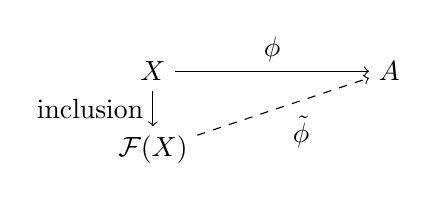
\begin{tikzpicture}
        \node at (0, 0) (X) {$X$};
        \node at (3, 0) (F) {$A$};
        \node at (0, -1) (A) {$\mathcal{F}(X)$};
        \draw[->] (X) -- node[above] {$\phi$} (F);
        \draw[->] (X) -- node[left] {inclusion} (A);
        \draw[->, dashed] (A) -- node[below right] {$\tilde{\phi}$} (F);
        \end{tikzpicture}.
\]
\end{property}


\begin{proposition}
\label{prop: free algebra hilbert series}
Given a sequence $\vec{a} = (a_{1}, a_{2}, \ldots)$ of nonnegative integers, let $X$ be a graded set with $|X_{i}| = a_{i}$, and consider the free algebra $\mathcal{F}(X)$.  Then the Hilbert series for $\mathcal{F}(X)$ is
\[
\mathrm{Hilb}(\mathcal{F}(X); t) =  \frac{1}{1 - a_{1}t - a_{2}t^{2} - a_{3}t^{3} - \cdots}.
\]
%
%
%
%Given a sequence $\vec{a} = (a_{1}, a_{2}, \ldots)$ of nonnegative integers, let $\mathfrak{L}(\vec{a})$ denote the free, graded Lie algebra with $a_{i}$ generators in degree $i$, and zero generators in degree zero.  The universal enveloping algebra
%\[
%\mathcal{U}\big(\mathfrak{L}(\vec{a})\big)
%\]
%
%\begin{enumerate}
%
%\item is a free, cocommutative, graded, connected Hopf algebra.
%
%\item has Hilbert series
%
%\[
%f(t)=\frac{1}{1 - a_{1}t - a_{2}t^{2} - a_{3}t^{3} - \cdots}.
%\]
%
%\end{enumerate}
\end{proposition}

\begin{proof}
%
%\begin{enumerate}
%
%    \item From Jacobson \cite[more specific reference]{jacobson2013lie}\lucas{This is now proved in section~\ref{sec:envelopingalgebras}, we should refer to this or remove this claim entirely.}
%
%    \item 
    Expand the following generating function as a geometric series, we have 

    $${\begin{split}
        \frac{1}{1 - a_{1}t - a_{2}t^{2} - a_{3}t^{3} - \cdots} &= \sum_{n=0}^\infty (a_1t+a_2t^2+\cdots)^n~.
    \end{split}}$$

    Expanding this sum we have the following equality

    $$\frac{1}{1 - a_{1}t - a_{2}t^{2} - a_{3}t^{3} - \cdots}
    =\sum_{n=0}^\infty \left(\sum_ {\beta \vDash n} a_\beta \right) t^n.$$

    Given $\Vec{a} = (a_{1}, a_{2}, \ldots)$, we can consider that $\mathfrak{L}(\Vec{a})$\mike{what is $\mathfrak{L}(\Vec{a})$?  Should this be
    $\mathcal{F}(X)$?}
is generated by the set
    $$X=\biguplus_{i \geq 1}\{x_{(i,j)}: 1 \leq j \leq a_i\}$$
     where for each $j$, $x_{(i,j)}$ is a generator of degree $i$.\mike{what do we mean ``is a generator''? of what?}

From ~\cite[Theorem 7 (Witt)]{jacobson2013lie} we have that a basis for the graded components $\mathcal{U}\big(\mathfrak{L}(\vec{a})\big)_n$ is the set of monomials of the form $m=x_{(\beta_1,j_1)} \cdots x_{(\beta_\ell,j_\ell)}$ where
     for each $d$, $1 \leq j_d \leq a_{\beta_{d}}$ with $\beta=(\beta_1,\dots,\beta_\ell)$ is a composition of $n$.
By counting the number of monomials of degree $n$,
we conclude that the dimension of each graded component of $\mathcal{F}(X)$
is given by $\sum_ {\beta \models n} a_\beta$
which is the coefficient of $t^n$ in the generating function.
%\end{enumerate}

\end{proof}

\subsection{Universal Enveloping Algebras}
\label{sec:envelopingalgebras}

Let $L$ be a graded Lie algebra with bracket $[\cdot, \cdot]$.  The universal enveloping algebra is the graded associative algebra on the space
\[
\mathcal{U}(L) = \bigoplus_{n \ge 0} \bigoplus_{\alpha \vDash n} L_{\alpha_{1}} \otimes L_{\alpha_{2}} \otimes \cdots \otimes L_{\alpha_{\ell}},
\]
where the degree zero component is $\CC 1_{\mathcal{U}(L)}$.
Multiplication in $\mathcal{U}(L)$ is concatenation of tensors,
subject to the relations of the form $a \otimes b - b \otimes a = [a, b]$
for all $a, b \in L$.  This algebra $\mathcal{U}(L)$ has the following \emph{universal property}:\mike{reference?}

\begin{property}
\label{prop:universalLie}
Let $A = \bigoplus_{n \ge 0} A_{i}$ be a graded algebra.  For every linear map $\psi: L \to A$ such that $\psi(L_{i}) \subseteq A_{i}$ and
\[
\psi([a, b]) = \psi(a)\psi(b) - \psi(b)\psi(a)
\qquad\text{for all $a, b \in L$},
\]
there exists a unique graded algebra homomorphism $\tilde{\psi}: \mathcal{U}(L) \to A$ such that $\tilde{\psi}|_{L} = \psi$, i.e.
\[
    \begin{tikzpicture}
        \node at (0, 0) (L) {$L$};
        \node at (3, 0) (U) {$A$};
        \node at (0, -1) (A) {$\mathcal{U}(L)$};
        \draw[->] (X) -- node[above] {$\psi$} (U);
        \draw[->] (X) -- node[left] {inclusion} (A);
        \draw[->, dashed] (A) -- node[below right] {$\tilde{\psi}$} (U);
        \end{tikzpicture}.
\]
\end{property}

Given a graded set $X = \biguplus_{i \ge 1} X_{i}$, we also define the free Lie algebra on $X$ to be the graded Lie algebra
\mike{what are the $h_x$?}
\[
\mathfrak{L}_{X} = \bigoplus_{n \ge 1} \bigoplus_{\alpha \vDash n} \CC\operatorname{-spanning}\{\text{brackets of $h_{x_{i_{1}}}, \ldots, h_{x_{i_{\ell}}}$} \;|\; x_{i_{k}} \in X_{\alpha_{k}} \},
\]
subject only to anticommutativity and the Jacobi identities.\mike{what are these relations?}

%The following is quoted word for word from \cite{jacobson2013lie}. Lie algebras arise from associative algebras in a very simple way. Let $A$ be an associative algebra. If $x,y,\in A$, then we define the \textit{Lie product} or (additive) \textit{commutator} of $x$ and $y$ as
%
%$$[x,y]=xy-yx.$$
%
%One checks immediately that
%
%$$\begin{matrix}
%    [x_1+x_2,y]=[x_1,y]+[x_2,y], \\
%    [x,y_1+y_2]=[x,y_1]+[x,y_2],\\
%    \alpha[x,y]=[\alpha x,y]=[x,\alpha y].
%\end{matrix}$$
%
%Thus the products $[x,y]$ satisfies all the conditions on the product in a Lie algebra. The Lie algebra obtained in this way is called \textit{the Lie algebra} of the associative algebra $\mathfrak{U}$. We shall denote this Lie algebra as $\mathfrak{U}_L$.

\begin{thm}[Theorem $7$ (Witt),\cite{jacobson2013lie}]
Let $X$ be an arbitrary graded set.  Then
\[
\mathcal{U}(\mathfrak{L}_{X}) \cong \mathcal{F}(X).
\]
\label{thm: free UEA}
%
%Let
%
%
%Let $X$ be an aribtrary set and let $\mathcal{F}$ denote the free algebra (freely) generated by $X$. Let $\mathfrak{F}^{\mathfrak{L}}$ denote the subalgebra of $\mathfrak{F}_L$ generated by the elements of $X$. Then $\mathfrak{F}^{\mathfrak{L}}$ is a free Lie algebra generated by $X$ and $\mathfrak{F}$ is the universal enveloping algebra of $\mathfrak{F}^{\mathfrak{L}}$. 
\end{thm}
\begin{proof}
    Let \(X = \biguplus_{n \ge 1} X_{n}\) be a graded set and let \(\mathcal{F}(X)\) be the free algebra generated by \(X\). Also, let \( \mathcal{U} (\mathfrak{L}_{X})\) be the Universal Enveloping algebra of the free Lie algebra generated by \(X\). 
    Define the map 
    \begin{align*}
        \begin{array}{rcl}
            \phi :  X \longrightarrow & \mathcal{U} (\mathfrak{L}_{X}) \\
             x  \longmapsto  & h_x \\ 
        \end{array}
    \end{align*}
    where \(h_x =  h_{x_{i_{1}} }h_{x_{i_{2}} }\cdots h_{x_{i_{k}} } \in \mathcal{U} (\mathfrak{L}_{X})\) is the product of formal generators in \(X\). 
    By Property~\ref{prop:universalfree} we have the unique graded homomorphism 
    \begin{align*}
        \begin{array}{rcl}
            \tilde{\phi}: \mathcal{F}(X) \longrightarrow & \mathcal{U} (\mathfrak{L}_{X}) \\
            g_x \longmapsto & h_x
        \end{array}
    \end{align*}
    where \(g_x = g_{x_{i_{1}} }g_{x_{i_{2}} }\cdots g_{x_{i_{\ell}} } \in \mathcal{F}(X)\) is also the product of formal generators in \(X\). Similarly, 
    define 
    \begin{align*}
        \begin{array}{rcl}
            \psi :  \mathfrak{L}_{X} \longrightarrow &\mathcal{F}(X) \\
        x  \longmapsto  & g_x .\\
        \end{array}
    \end{align*}
    From Property~\ref{prop:universalLie} we obtain another unique graded homomorphism 
    \begin{align*}
        \begin{array}{rcl}
            \tilde{\psi}: \mathcal{U}(\mathfrak{L}_{X}) \longrightarrow & \mathcal{F} (X) \\
            h_x \longmapsto & g_x.
        \end{array}
    \end{align*}
    To see that \(\mathcal{U}(\mathfrak{L}_{X}) \cong \mathcal{F}(X)\), notice that
    \begin{align*}
        \tilde{\phi}(\tilde{\psi}(h_{x_{i_{1}} }h_{x_{i_{2}}} \cdots h_{x_{i_{k}}}))  
        &= \tilde{\phi}(\tilde{\psi}(h_{x_{i_{1}} })\tilde{\phi}(\tilde{\psi}(h_{x_{i_{2}} } )\cdots \tilde{\phi}(\tilde{\psi}(h_{x_{i_{k}} })) \\
        &=  \tilde{\phi}(g_{x_{i_{1}} })\tilde{\phi}(g_{x_{i_{2}} })\cdots \tilde{\phi}(g_{x_{i_{\ell}} })\\
        &= h_{x_{i_{1}} }h_{x_{i_{2}} } \cdots h_{x_{i_{k}} }
    \end{align*} 
    Similarly, it can also be shown that \(\tilde{\psi} \circ \tilde{\phi} (g_x) = g_x\) and as such \(\tilde{\phi} \circ \tilde{\psi} = \tilde{\psi} \circ \tilde{\phi} = id\).
    Therefore, since \(\tilde{\phi}\) and \(\tilde{\psi}\) are inverses of each other,  \(\mathcal{U}(\mathfrak{L}_{X}) \cong \mathcal{F}(X)\).
\end{proof}

%Let $\Phi$ be a field. For the sake of simplcity we shall now restrict our attention to the case of a finite set set $X=\{x_1,x_2,\cdots,x_r\}$. Then
%define
%$$\mathfrak{M}:=\Phi x_1 \oplus \Phi x_2 \oplus \cdots \oplus \Phi x_r$$
%
%and $\mathfrak{F}= \Phi 1 \oplus \mathfrak{M} \oplus (\mathfrak{M} \otimes \mathfrak{M}) \oplus \cdots$, and we write $\mathfrak{F}=\Phi\{x_1,\ldots,x_r\}$. The algebra $\mathfrak{F}$ is graded with $\mathfrak{M}_m=\mathfrak{M}\otimes\mathfrak{M}\otimes\cdots \otimes \mathfrak{M}$ ($m$-times) as the space of the homogeneous elements of degree $m$. A basis for this space is the set of monomials of the form $x_{i_1}x_{i_2}\cdots x_{i_m}$, $i_j=1,2,\cdots,r$; hence $\dim \mathfrak{M}_m=r^m$.

\section{Characterization of \textsf{FGCCHA}s by $a$ sequences}

The structure of a connected cocommutative Hopf algebra is completely determined by certain elements called \textit{primitives}.
\begin{definition}
    An element $p$ is \textit{primitive} if $\Delta(p) = 1 \otimes p + p \otimes 1$. The primitives of a Hopf algebra $H$ will be denoted $\mathcal{P}(H)$.
\end{definition}

Under the commutator bracket, $\mathcal{P}(H)$ forms a graded Lie algebra. For a Lie algebra $L$, $\mathcal{U}(L)$ has a cocommutative Hopf algebra structure, with the coproduct $\Delta_L$ induced by the map
\[
\delta :L\to \mathcal{U}(L)\otimes\mathcal{U}(L) \text{  with  }\delta(x)=1\otimes x + x\otimes 1.
\] 
It follows from \cite[Theorem 1.4]{Reutenauer-FreeLieAlgebras} that under this coproduct, $\mathcal{P}(\mathcal{U}(L))=L$.
The Cartier-Milnor-Moore theorem~\cite[see Theorem 5.18]{MM65} characterizes a connected cocommutative Hopf algebra $H$ by its primitive elements,
\[
\mathcal{U}(\mathcal{P}(H))\cong H.
\]
In the case that $H$ is a connected cocommutative Hopf algebra freely generated by a graded set $X$, 
we will further demonstrate that $H\cong \mathcal{U}(\mathfrak{L}_X).$

To begin, we will construct a set of free primitive generators for $H$.  
Our methods generalize those of Lauve-Mastnak in \cite{LM11}, and also follow from~\cite[Prop. 9.9]{S94} which make use of the \emph{Eulerian idempotent}
\[
\mathbf{e} = \sum_{k \geq 1}\frac{(-1)}{k}^{k-1} \mu^{(k-1)} \circ \tilde{\Delta}^{(k-1)},
\]
which projects onto $\mathcal{P}(H)$ for a connected cocommutative Hopf algebra $H$ \cite[Theorem 9.4]{S94}.

\begin{lemma}
\label{lemma:primitive generators}
    Let $H$ be a graded connected cocommutative Hopf algebra, freely generated by a graded set $X=\biguplus_{n \geq 1}X_n$.  Then the graded set
    \[
    \mathbf{e}(X) = \biguplus_{n \ge 1} \{\mathbf{e}(x) \;|\; x \in X_{n}\}
    \]
    comprises a complete set of primitive generators of $H$.
\end{lemma}
\begin{proof}
    We will first show $\mathbf{e}(X)$ is algebraically independent in $H$. Fix a total order in each $X_n$, and extend to a total order on $X$, such that if $x\in X_i, y\in X_j$ and $i>j$, then $x<y$. For any $x\in X$, we have
    \[
    \mathbf{e}(x) = \text{id} (x) - \frac{1}{2}\mu \circ \tilde{\Delta}(x) + \cdots = x + p((x_i)),
    \]
    where $p((x_i))$ is some polynomial in generators $x_i$ of lesser degree than $x$. Then the minimal term in $\mathbf{e}(x)$ is $x$, and any polynomial $q(\mathbf{e}(x_1),...,\mathbf{e}(x_n))$ has the same minimal term as $q(x_1,...,x_n)$. Hence if $f$ is a non-trivial polynomial and $f(\mathbf{e}(x_1), \ldots, \mathbf{e}(x_n)) = 0$, then $f(x_1, \ldots, x_n) = 0$, a contradiction. Therefore $\mathbf{e}(X)$ is an algebraically independent set.

    To show $\mathbf{e}(X)$ generates $H$, observe that in each degree $n$, the monomials in $X$ of degree $n$ form a basis for $H_n$. The degree $n$ monomials in $\mathbf{e}(X)$ are linearly independent, because the $\mathbf{e}(X)$ are algebraically independent. Because every monomial $\mathbf{e}(x_1)\mathbf{e}(x_2)\cdots \mathbf{e}(x_k)$ corresponds uniquely to the monomial $x_1x_2 \cdots x_k$, the degree $n$ monomials in $\mathbf{e}(X)$ form a basis of $H_n$, hence $\mathbf{e}(X)$ freely generates $H$.
\end{proof}

We may now present the main result of this section.

\begin{theorem}
\label{thm: Hopf dimension isomorphic}
    For every non-negative sequence $(a_n)_{n \geq 1}$ there exists a \textsf{FGCCHA} with $a_n$ generators in degree $n$, unique up to isomorphism.
\end{theorem}

\begin{proof}
    For a sequence of non-negative integers $(a_n)_{n \geq 1}$, the Hopf algebra $\mathcal{U}(\mathfrak{L}(\vec{a}))$ has $a_n$ generators in degree $n$.

    To show uniqueness, suppose $H$ and $K$ are two \textsf{FGCCHA}s with $a_n$ generators in degree $n$. Choose homogeneous generating sets $X\subseteq H$ and $Y \subseteq K$, then $\mathbf{e}(X)$ and $\mathbf{e}(Y)$ are free primitive generators of each Hopf algebra. We may choose a bijection $f:\mathbf{e}(X) \to \mathbf{e}(Y)$ that respects grading, i.e. $f(\mathbf{e}(X_n)) = \mathbf{e}(Y_n)$. Extending algebraically we have a graded algebra isomorphism $\tilde{f}:H \to K$, and because $\mathbf{e}(X)$ and $\mathbf{e}(Y)$ are primitives $\tilde{f}$ is a graded Hopf algebra isomorphism.
\end{proof}

\begin{corollary}
    Suppose $H$ and $K$ are \textsf{FGCCHA}s with $\dim(H_n) = \dim(K_n)$ for all $n \geq 0$. Then $H \cong K$.
\end{corollary}

\begin{proof}
    By \ref{prop:sequences}, $H$ and $K$ have the same $a$-sequence, hence they are isomorphic by \ref{thm: Hopf dimension isomorphic}.
\end{proof}

We will now state some results which will be useful later in the paper.

\begin{proposition}~\cite[Prop. 2.4]{F23}
\label{prop:free primitives}
    Let $L$ be a Lie algebra, and suppose $\mathcal{U}(L)$ is freely generated by $X\subseteq L$. Then $L\cong \mathfrak{L}_X$.
\end{proposition}

\begin{proof}
   From Theorem~\ref{thm: free UEA} we have $\mathcal{U}(L) \cong \mathcal{F}(X) \cong \mathcal{U}(\mathfrak{L}_X)$ as algebras. Let $f:\mathcal{U}(L) \to \mathcal{U}(\mathfrak{L}_X)$ be the isomorphism extending $f(x)=h_x$ for generators $x \in X$. The generators of each algebra are elements of their respective Lie algebras, hence 
    \[
    \Delta_{\mathfrak{L}_X} \circ f(x)=1 \otimes f(x) + f(x) \otimes 1 = f \otimes f \circ \Delta_L(x) 
    \]
    for all $x \in X$. By extension $f:\mathcal{U}(L) \to \mathcal{U}(\mathfrak{L}_X)$ is a bialgebra isomorphism, therefore
    \[
    L \cong \mathcal{P}(\mathcal{U}(L)) \cong \mathcal{P}(\mathcal{U}(\mathfrak{L}_X)) \cong \mathfrak{L}_X.
    \]
\end{proof}

\begin{corollary}
    Let $H$ be a graded connected cocommutative Hopf algebra freely generated by $X$. Then $H \cong \mathcal{U}(\mathfrak{L}_X)$ and $\mathcal{P}(H)\cong \mathfrak{L}_X.$
\label{cor: free hopf primitives}
\end{corollary}
\begin{proof}
    By Lemma~\ref{lemma:primitive generators} we may choose $X'\subseteq \mathcal{P}(H)$ freely generating $H$. By Prop.~\ref{prop:free primitives}, $H\cong \mathcal{U}(\mathfrak{L}_{X'})$ hence $\mathcal{P}(H)\cong \mathfrak{L}_{X'}\cong \mathfrak{L}_X.$
\end{proof}

\section{Classification of free cocommutative graded connected Hopf algebras} 

Given a sequence $\vec{a} = (a_{1}, a_{2}, \ldots)$ of nonnegative integers, let $\mathfrak{L}(\vec{a})$ denote the free, graded Lie algebra with $a_{i}$ generators in degree $i$, and zero generators in degree zero.  The universal enveloping algebra
\[
\mathcal{U}\big(\mathfrak{L}(\vec{a})\big)
\]
is a cocommutative, graded, connected Hopf algebra, and we have shown that it is free, with Hilbert series
\[
\frac{1}{1 - a_{1}t - a_{2}t^{2} - a_{3}t^{3} - \cdots}.
\]

%\begin{thm}
%Let $H=\bigoplus_{n\geq 0} H_n$ and $K=\bigoplus_{n\geq 0} K_n$ be two free graded connected cocommutative Hopf algebras. The following are equivalent.
%\begin{enumerate}
%\item $H\cong K$ as graded Hopf algebras. 
%
%\item $\dim(H_n)=\dim(K_n) \text{ for all } n\geq 0.$
%\end{enumerate}   
%\end{thm}
%
%\begin{proof}
%Immediately we have (1)$\Rightarrow$(2). Assume that $\dim(H_n)=\dim(K_n) \text{ for all } n\geq 0,$
%or equivalently $\mathcal{H}(H;t)=\mathcal{H}(K;t).$
%Since both $H$ and $K$ are both freely generated, there exist graded sets
%$X$ and $Y$ generating $H$ and $K$, respectively.
%Define the series $\mathcal{G}(X;t)=\sum_{n\geq 0}|X_n|t^n$.
%It follows from Proposition \ref{prop: free algebra hilbert series}
%\mike{is this right?  I found "Prop. 3.2" in the text and
%it no longer referred to the correct thing} that
%\[
%\mathcal{H}(H;t)=\frac{1}{1-\mathcal{G}(X;t)}\ \text{  and  }\ \mathcal{H}(K;t)=\frac{1}{1-\mathcal{G}(Y;t)}.
%\]
%Because $H$ and $K$ are connected, the degree zero terms of their Hilbert series $\dim(H_0)=\dim(K_0)=1$ are non-zero, hence the following equality of series
%\[
%\mathcal{G}(X;t)=1-\frac{1}{\mathcal{H}(H;t)}=1-\frac{1}{\mathcal{H}(K;t)}=\mathcal{G}(Y;t).
%\]
%We then have $|X_i|=|Y_i|$ for all $i\geq 0.$ Fix bijections $\varphi_i:X_i\to Y_i$ and extend
%to a bijection $\varphi:X\to Y$. This graded bijection of generating sets induces a graded
%Lie algebra isomorphism $\hat{\varphi}:\mathfrak{L}_X\to \mathfrak{L}_  Y$.\mike{How? reference?}
%From Corollary~\ref{cor: free hopf primitives} we have
%\[
%\mathcal{P}(H)\cong \mathfrak{L}_X \text{ and } \mathcal{P}(K)\cong \mathfrak{L}_Y.
%\]
%We conclude by the Cartier-Milnor-Moore\mike{reference?} theorem that
%\[
%H\cong \mathcal{U}(\mathfrak{L}_X)\cong \mathcal{U}(\mathfrak{L}_Y)\cong K.
%\]
%\end{proof}


\begin{thm}[Various Sources]
Let $H$ be a free, cocommutative, graded, connected Hopf algebra, and let $\vec{a} = (a_{1}, a_{2}, \ldots, )$ count the number of free generators of $H$ in each degree.  
\begin{enumerate}
\item There is a graded isomorphism $H \cong \mathcal{U}\big(\mathfrak{L}(\vec{a})\big)$ of Hopf algebras.

\item Every graded sub-Hopf algebra of $H$ is isomorphic to $\mathcal{U}\big(\mathfrak{L}(\vec{b})\big)$ for some sequence $\vec{b} = (b_{1}, b_{2}, \ldots)$.

\item For every sequence $\vec{b} = (b_{1}, b_{2}, \ldots)$ with $b_{i} \le a_{i}$, $H$ has a graded sub-Hopf algebra isomorphic to $\mathcal{U}\big(\mathfrak{L}(\vec{b})\big)$.

\end{enumerate}
\end{thm}
\begin{proof}
Here is a sketch of what we need to formalize:
\begin{enumerate}
\item %Using Aliniaeifard--Thiem's result~\cite[Theorem 4.2]{AT22}, we only need to compare the Hilbert series of $H$ and $\mathcal{U}\big(\mathfrak{L}(\vec{a})\big)$ to prove this part.  \lucas{Should we write out their proof to convince ourselves it is true.  It is short.}

Following Aliniaeifard--Thiem's result~\cite[Theorem 4.2]{AT22}, one only need to compare the Hilbert series of $H$ and $\mathcal{U}\big(\mathfrak{L}(\vec{a})\big)$.


\item Let $G \subseteq H$ be a sub-Hopf algebra.  By (1), the Lie algebra of primitives $\mathcal{P}(H) \cong \mathcal{L}(\vec{a})$.  Thus $\mathcal{P}(G)$ is isomorphic to a subalgebra of $\mathcal{L}(\vec{a})$.  

By~\cite[Theorem 2.2]{MSZ}, $\mathcal{P}(G)$ is a free Lie algebra, so there exists a sequence $\vec{b} = (b_{1}, b_{2}, \ldots)$ for which $\mathcal{P}(G) \cong \mathfrak{L}(\vec{b})$.
%\lucas{Detail: show that this result plays well with the grading?}  
By Milnor--Moore, $G \cong \mathcal{U}\big(\mathfrak{L}(\vec{b})\big)$.

%Missing: what can we say about $\vec{b}$, i.e. the rank of $\mathcal{P}(G)$?  I really think it should satisfy $b_{i} \le a_{i}$, but free objects are weird so this needs a proof\lucas{Big detail!! This actually seems to be false}.  Since we are wrong here, we still could have a classification of sub-Hopf algebras by sequences $\vec{b}$, but we would need to figure out the correct constraints on $\vec{b}$.

\item Here, we construct $\mathfrak{L}(\vec{b})$ as a subalgebra of $\mathfrak{L}(\vec{a})$ by taking $b_{i}$ of the free generators in degree $i$.
\end{enumerate}
\end{proof}

Previously, we had thought that the condition in (3) above was sufficient, i.e. that every graded sub-Hopf algebra of $\mathcal{U}\big(\mathfrak{L}(\vec{a})\big)$ was isomorphic to $\mathcal{U}\big(\mathfrak{L}(\vec{b})\big)$ for some sequence $(b_{1}, b_{2}, \ldots)$ with $0 \le b_{i} \le a_{i}$ for all $i \ge 1$.  However, this is not true!  

Consider the free, connected, cocommutative Hopf algebra which is freely generated as an algebra by four homogeneous elements of degree one, $x$, $y$, $z$, and $w$, so that
\[
H_{1} = \CC\operatorname{-span}\{x, y, z, w\}
\]
and
\[
H_{k} = \CC\operatorname{-span}\big\{ \text{products $m_{1} m_{2} \cdots m_{k}$} \;|\; m_{i} \in \{x, y, z, w\} \big\}
\qquad\text{for $k \ge 2$}.
\]
By Proposition~\ref{prop: free algebra hilbert series}, $H$ has the Hilbert series
\[
\frac{1}{1 - 4t - 0 t^{2} - 0 t^{3} - \cdots }.
\]

The Lie algebra of primitives $\mathcal{P}(H)$ is the free Lie algebra $\mathfrak{L}_{\{x, y, z, w\}}$.  Now consider the Lie subalgebra
\[
M = \CC\operatorname{-span}\{[x, y]\} \subseteq \mathfrak{L}_{\{x, y, z, w\}},
\]
as well as its universal enveloping algebra $\mathcal{U}(M) \subseteq H$.
By Theorem~\ref{}, this is a free Lie algebra generated by one element, and by dimension consideration we can take the free generator to be $[x, y]$.  
Therefore by Theorem~\ref{}, the universal enveloping algebra $\mathcal{U}(M)$ is freely generated (as an algebra) by $[x, y]$.
Now $[x, y] = xy - yx$ is a homogeneous element of degree $2$ in $H$, so as the subalgebra generated by $[x, y]$, the universal enveloping algebra $\mathcal{U}(M)$ is a graded sub-Hopf algebra and has Hilbert series
\[
\frac{1}{1 - 0t - t^{2} - 0t^{3} - \cdots}.
\]
Since $H$ has no free generators in degree $2$, this shows that sub-Hopf algebras may have more free generators in a given degree than the Hopf algebra which contains them.

Is is also possible to obtain a sub-Hopf algebra which has more free generators (in total) than the Hopf algebra which contains it.  
Consider the Lie subalgebra
\[
N = \langle [x, y], [x, z], [x, w], [y, z], [y, w], [z, w] \rangle \subseteq \mathfrak{L}_{\{x, y, z, w\}}.
\]
This is free on the set $\{[x, y], [x, z], [x, w], [y, z], [y, w], [z, w]\}$.  \lucas{Definitely true, but details needed.}  Repeating the argument we made for $\mathcal{U}(M)$, we have that $\mathcal{U}(N)$ is a graded sub-Hopf algebra of $H$ with six free generators in degree two, so that its Hilbert series is
\[
\frac{1}{1 - 0t - 6t^{2} - 0 t^{3} - \cdots }.
\]

\begin{question}
Let $\vec{a} = (a_{1}, a_{2}, \ldots)$ be a sequence of nonnegative integers.  What characterizes the sequences $\vec{b} = (b_{1}, b_{2}, \ldots)$ for which $\mathcal{U}(\mathfrak{L}(\vec{a}))$ has a graded sub-Hopf algebra isomorphic to $\mathcal{U}(\mathfrak{L}(\vec{b}))$?
\end{question}



Given a sequence $\vec{a} = (a_1,a_2, \ldots)$ we have a formula for the dimension of the free Lie algebra with $a_i$ generators in each degree $i$~\cite[Theorem 2.2]{KK95}:
\[
\dim \mathfrak{L}(\vec{a})_n = \sum_{mk=n} \frac{1}{k}\mu (k) \mathbf{W}_m(\vec{a})
\]
where $\mu$ is the Mobius function, and setting $\lambda^!$ to be the multipllicity factorial and $\ell(\lambda)$ the length of $\lambda$,
\[
\mathbf{W}_m(\vec{a}) = \sum_{\lambda \vdash m} \frac{(\ell(\lambda)-1)!}{\lambda^!}a_{\lambda_1} \cdots a_{\lambda_{\ell}}.
\]
Define 
\[
P_n(\vec{a}) = \sum_{mk=n} \frac{1}{k}\mu (k) \mathbf{W}_m(\vec{a})
\]
so that $P_n(\vec{a}) = \dim \mathfrak{L}(\vec{a})_n$.

\begin{theorem}
\label{thm:subclassification1}
    Let $\vec{a} = (a_{1}, a_{2}, \ldots)$ and $\vec{b} = (b_{1}, b_{2}, \ldots)$ be sequences of nonnegative integers. The following are equivalent.
    \begin{enumerate}
        \item $\mathcal{U}(\mathfrak{L}(\vec{a}))$ has a sub-Hopf algebra isomorphic to $\mathcal{U}(\mathfrak{L}(\vec{b}))$
        \item $\mathfrak{L}(\vec{a})$ has a sub-Lie algebra isomorphic to $\mathfrak{L}(\vec{b})$.
        \item $P_n(\vec{a}) \geq P_n(\vec{b})$ for all $n > 0$.
    \end{enumerate}
\end{theorem}

\begin{proof}
    The equivalence of (1) and (2) is clear. We will show (2) and (3) are equivalent. Suppose $\mathfrak{L}(\vec{a})$ has a sub-Lie algebra isomorphic to $\mathfrak{L}(\vec{b})$. Then
    \[
    P_n(\vec{b}) = \dim \mathfrak{L}(\vec{b})_n \leq \dim \mathfrak{L}(\vec{a})_n = P_n(\vec{a}).
    \]

    Now suppose $P_n(\vec{a}) \geq P_n(\vec{b})$ for all $n > 0$. We will construct a sub-Lie algebra $B \subseteq \mathfrak{L}(\vec{a})$ isomorphic to $\mathfrak{L}(\vec{b})$ by recursively choosing $b_n$-dimensional subspaces complementary to $[B,B]_n$ in each degree $n$. Let $V \subseteq \mathfrak{L}(\vec{a})$ be the subspace spanned by the free generators, so that $\mathfrak{L}(\vec{a}) = V \oplus [\mathfrak{L}(\vec{a}),\mathfrak{L}(\vec{a})]$. Note that we can recursively define 
    \[ 
    [B,B]_n = \sum_{k=1}^{n-1} [B_k,B_{n-k}].
    \]

    For $n=1$ we have $P_1(\vec{a}) = a_1$ and $P_1(\vec{b}) = b_1$, hence $a_1 \geq b_1$. Let $W_1$ be the span of $b_1$ of the degree 1 generators. Trivially $W_1$ is complementary to $[B,B]_1 = \{0\}.$
    Suppose in each degree $1 \leq k < n$ we have chosen subspaces $W_k$ complementary to $[B,B]_k$. If $b_n \leq a_n$ we may simply choose a $b_n$-dimensional subspace of $V_n$. Otherwise, suppose $b_n > a_n$. Because $\mathfrak{L}(\vec{a})_n = V_n \oplus [\mathfrak{L}(\vec{a}),\mathfrak{L}(\vec{a})]_n$, we have
    \[
    \dim [\mathfrak{L}(\vec{a}),\mathfrak{L}(\vec{a})]_n = \dim \mathfrak{L}(\vec{a}) - \dim V_n = P_n(\vec{a}) - a_n.
    \]
    Because the spaces $B_k = W_k \oplus [B,B]_k$ are defined for $1 \leq k < n$, the space $[B,B]_n$ is defined recursively. Furthermore, $[B,B]_n$ is a subspace of $[\mathfrak{L}(\vec{a}),\mathfrak{L}(\vec{a})]_n$.
    \\
    \textit{Claim.} $\dim [B,B]_n = P_n(\vec{b}) - b_n$.
    \\                    
    
    Given the claim, we have
    \[
    \dim \frac{[\mathfrak{L}(\vec{a}),\mathfrak{L}(\vec{a})]_n}{[B,B]_n} = P_n(\vec{a}) - a_n - \dim [B,B]_n \geq P_n(\vec{a}) - P_n(\vec{b}) + b_n - a_n \geq b_n - a_n. 
    \]
    Then we may choose $b_n - a_n$ linearly independent elements of $\frac{[\mathfrak{L}(\vec{a}),\mathfrak{L}(\vec{a})]_n}{[B,B]_n}$, and together with the $a_n$ generators in degree $n$ they span a $b_n$-dimensional subspace $W_n$ complementary to $[B,B]_n.$ Thus we have recursively defined 
    \[
    B = \bigoplus_{n\geq 1}W_n \oplus [B,B]_n = W \oplus [B,B].
    \]
    with $W = \bigoplus_{n\geq 1} W_n$ and $\dim W_n = b_n$.
    
    Clearly $B$ is closed under the Lie bracket, and is a sub-Lie algebra of $\mathfrak{L}(\vec{a}).$ By the Shirshov-Witt Theorem ~\cite[text]{S09}, $B$ is a free Lie algebra and is therefore generated by a basis for $W$, hence $B \cong \mathfrak{L}(\vec{b}).$
\end{proof}

\begin{proof}[Proof of Claim]
Let $W_k$ be defined as above for $1 < k < n.$ Set $W_{<n} = \bigoplus_{k=1}^{n-1} W_k$ and let $\mathfrak{L}(W_{<n})$ be the free Lie algebra on $W_{<n}$  (this is equivalent to the free Lie algebra generated by a basis for $W_{<n}$). Since $\mathfrak{L}(W_{<n}) = W_{<n} \oplus [\mathfrak{L}(W_{<n}) , \mathfrak{L}(W_{<n})]$, we have $\mathfrak{L}(W_{<n})_1 = W_1 = B_1$, and recursively for $1 < k <n$ we have
\[
\mathfrak{L}(W_{<n})_k = W_k \oplus [\mathfrak{L}(W_{<n}) , \mathfrak{L}(W_{<n})]_k = W_k \oplus [B,B]_k = B_k
\]
therefore $[B,B]_n = [\mathfrak{L}(W_{<n}),\mathfrak{L}(W_{<n})]_n$.

Define the sequence $\vec{b} \vert_n = (b_1,b_2, \ldots , b_{n-1}, 0, \ldots)$. Then $\dim \mathfrak{L}(W_{<n})_n = P_n(\vec{b}|_n)$. Because the only term of 
\[ 
P_n(\vec{b}) = \sum_{mk=n} \frac{1}{k}\mu (k) \sum_{\lambda \vdash m} \frac{(\ell(\lambda)-1)!}{\lambda^!}b_{\lambda_1} \cdots b_{\lambda_{\ell}}
\]
containing $b_n$ is with $m = n$ and $\lambda = (n)$ with a coefficient of $1$, we have $P_n(\vec{b}|_n) = P_n(\vec{b}) - b_n$. Therefore
\[
\dim [B,B]_n = \dim [\mathfrak{L}(W_{<n}),\mathfrak{L}(W_{<n})]_n = P_n(\vec{b}|_n) = P_n(\vec{b})-b_n.
\]
\end{proof}

\section{A set of details to add}

Aliniaeifard-Thiem \cite[Theorem 4.2]{AT22} give a theorem that says that two co-commutative Hopf algebras that
have the same sequence of graded dimensions are isomorphic.  We should have a section here
that says how to carry out this construction (outlined in the Cocalc summary for July 3).

Let \(H\) and \(K\) be two free graded cocommutative Hopf algebras, such that \(\dim(H_n) = \dim(K_n)\) for all \(n \geq 0\).
Aliniaeifard-Thiem  ~\cite[Theorem 4.2]{AT22}, guarantees that \(H \cong K\) and we outline here the method for constructing an 
isomorphism \(f:H \to K\).  In general, the idea is to find the free primitive generators of \(H\) and \(K\), and map the primitive generators of 
each graded component \(H_n\) to the primitive generators of the  coresponding graded component \(K_n\).

Aguiar-Lauve \cite{AL15} give the Eulerian idempotent operator
\[
    \mathbf{e} = \sum_{k=1}^\infty \frac{(-1)^{k-1}}{k} m^{(k-1)}\circ \Delta^{(k-1)}
\]
which for any cocommutative Hopf algebra projects onto the space of primitive elements. Since \(H\) and \(K\) are cocommutative
we can use \(\mathbf{e}\) to compute  \(\mathcal{P}(H)\) and \(\mathcal{P}(K)\).
Then, by ~\ref{lemma:primitive generators}, there exists \(X \subseteq \mathcal{P}(H)\) such that \(H\) is generated by \(X\)
and  \(Y \subseteq \mathcal{P}(K)\) such that  \(K\) is  generated by \(Y\).

In order to distinguish the free primitive generators \(X\)
from the primitive elements \(\mathcal{P}(H)\) consider the decomposition \[
    \mathcal{P}(H) = V \oplus [\mathcal{P}(H), \mathcal{P}(H)]
\] where \([\mathcal{P}(H), \mathcal{P}(H)] = \CC\operatorname{-span}\{[p1,p2] \: \vert \: p_i \in \mathcal{P}(H)\}\) and
\(V\) is a graded subspace of \(\mathcal{P}(H)\). Since \(\mathcal{P}(H)\) forms a Lie algebra under the commutator bracket,
then, by ~\cite[Prop 2.2]{F23}, \(\mathcal{P}(H)\) is generated by a basis of \(V\). Hence \(X\) is a basis of \(V\). Therefore, in general,
to find the set of primitive generators of \(H\), first choose a graded subspace \(V \subseteq \mathcal{P}(H)\), then choose a basis for \(V\).
Alternatively, letting \(V = \frac{\mathcal{P}(H)}{[\mathcal{P}(H), \mathcal{P}(H)]}\),
 any subset \(X' \subseteq \mathcal{P}(H)\) that descends to a basis of \(V\), will be a set primitive generators of \(H\).

Let \(p_i\) be a basis of \(V\) and let  \(A \in GL_{|I|}(\CC)\) be an invertible linear transformation.
Then, for some  \(b_i \in [\mathcal{P}(H), \mathcal{P}(H)]\),
we can characterize all possible bases for \(V\) as \[
    q_i = \sum_jA_{ij}p_i + b_i.
\]
Hence we find the free primitive generators \(X\) of \(H\) and \(Y\) of \(K\), and, as in the proof of
\cite{AT22}, fix bijections \(f_i: X_i  \to Y_i\) and extend to a bijection
\(f:X \to Y\).

\section{Classification by Sequences}

In this section we will characterize free graded connected cocommutative Hopf algebras in terms of sequences. For such a Hopf algebra $H$, we will denote
\begin{itemize} 
    \item $\vec{h} = (h_1, h_2, \ldots)$ where $h_n = \dim H_n$,
    \item $\vec{p} = (p_1, p_2, \ldots)$ where $p_n = \dim P(H)_n$,
    \item $\vec{a} = (a_1, a_2, \ldots)$ where $a_n$ is the number of generators in degree $n$.
\end{itemize}

\begin{proposition}
    The sequences above obey the following relations:
    \begin{itemize}
        \item[i)] $\displaystyle h_n
        = \sum_{\beta \vDash n} a_\beta
        = \sum_{\lambda \vdash n} \prod_{d \geq 1} \binom{p_d + m_d(\lambda) -1}{p_d -1}$
        \item[ii)] $\displaystyle p_n
        = \sum_{d|n} \sum_{\beta \vDash d} \frac{d\cdot \mu(n/d)}{n \cdot \ell(\beta)} a_\beta
        = \sum_{d|n} \sum_{\beta \vDash d} \frac{d\cdot \mu(n/d) (-1)^{\ell(\beta)-1}}{n \cdot \ell(\beta)} h_\beta$
        \item[iii)] $\displaystyle a_n
        = \sum_{\beta \vDash n} (-1)^{\ell(\beta)-1} h_\beta
        = \sum_{\lambda \vdash n} (-1)^{\ell(\lambda)-1} \prod_{d \geq 1} \binom{p_d}{m_d(\lambda)}~$
    \end{itemize}
\end{proposition}
\begin{proof}

By proposition \ref{prop:sequences},
it suffices to show that \eqref{eq:gf_relation} holds. The number of monomials of degree m is  $\displaystyle 
        \sum_{\beta \vDash m} a_\beta = \sum_{k\geq 0} \sum
    \limits_{\substack{\beta \vDash m \\ l(\beta)=k } }a_\beta $. Therefore, the Hilbert series associated to H is
 
\[ \sum_{k\geq 0} (\sum
    \limits_{\substack{\beta \vDash m \\ l(\beta)=k } }a_\beta t^m)=
   \sum_{k \geq 0} \left(\sum_{m \geq 1} a_m t^m\right)^k
   \]
   which in turn is equal to 
$\frac{1}{1 - \sum_{m \geq 1} a_m t^m}$
 using the expansion $\frac{1}{1-x}= \sum_{k\geq 0} x^k $.

On the other hand, each monomial of degree $m$ is a product of primitive generators. Therefore the number of polynomials of degree $m$ is the number of solutions to the equation $\sum\limits_{\substack {d}}\sum\limits_{\substack{ 1\leq i\leq p_d}}  c_{d_i}d=m$. The generating function associated to this equation is
$\prod_{d \geq 1} \frac{1}{(1-t^d)^{p_d}}$ where the number of integer solutions to the equation is the coefficient of $t^m$. It follows that 
\[
1 + \sum_{k \geq 1} h_k t^k=
\frac{1}{1 - \sum_{m \geq 1} a_m t^m}=
\prod_{d \geq 1} \frac{1}{(1-t^d)^{p_d}}.\]

\end{proof}
\begin{proposition}
\label{prop:h sequence}
	Given a sequence of nonnegative integers $\vec{h} = (h_0, h_1, h_2, \ldots)$, there exists a free graded connected cocommutative Hopf algebra $H$ with $\dim(H_n) = h_n$ for all $n \geq 0$ if and only if 
	
	$$a_n = \sum_{\beta \vDash n} (-1)^{\ell(\beta)-1} h_{\beta_{1}} \cdots h_{\beta_{\ell}} \geq 0 \text{ for all } n \geq 0.$$
	
	Moreover, if this is the case, then $H \cong \mathcal{U}(\mathfrak{L}(\vec{a}))$.	
%	Following this we can construct the Hopf algebra associated to it.
\end{proposition}

\begin{proof}

Suppose that we have a free, graded, connected, cocommutative Hopf algebra $H$ with $\dim(H_{i}) = h_{i}$.  Then by Proposition~\ref{prop:sequences}, $H$ is freely generated by a graded set $X = \biguplus_{i \ge 0} X_{i}$ with $|X_{i}| = a_{n}$ for each $n \ge 0$, and therefore $a_{n} \ge 0$.

On the other hand, assuming \(a_n \geq 0\) for all \(n \geq 0\), as a non-negative graded set, \(a_n\) generates a free graded connected cocommutative Hopf algebra \(H\). By Proposition~\ref{prop:sequences}  we have that  \(\vec{a}\) also corresponds to 
\(\vec{h} = (h_0, h_1, h_2, \ldots)\), where \(h_n \geq 0\) for all \(n \geq 0\) and \(\dim{H_n} = h_n\). 
Furthermore, \(H \cong \mathcal{U}(\mathfrak{L}(\vec{a}))\) by Corollary~\ref{cor: free hopf primitives}.
%	Suppose that $h_n$ correspond to the dimension of a free cocommutative graded connected Hopf algebra $H$ at degree $n$. By freeness, there exist graded sets X generating $H$. Theorem $1$, followed by Corollary $3.6$ gives us that $\mathcal{F}(X) \cong H$. From Proposition $3.2$ we then have that the dimension of each graded component of $\mathcal{F}(X)$, is given by $h_n=\sum_ {\alpha \models n} a_{\alpha_1} a_{\alpha_2} ... a_{\alpha_\ell}$. After manipulation, this gives us that 
%	\[
%	a_n = \sum_{\beta \vDash n} (-1)^{\ell(\beta)-1} h_{\beta_1} h_{\beta_2} \cdots h_{\beta_{\ell(\beta)}}.
%	\]
%We also have that the $a_n$ are nonnegative integers since they correspond to the number of free generators at degree $n$. 
%
%Now suppose that $a_n = \sum_{\beta \vDash n} (-1)^{\ell(\beta)-1} h_{\beta_1} h_{\beta_2} \cdots h_{\beta_{\ell(\beta)}}$ such that $a_n\geq 0$, by Theorem $1$, followed by Corollary $3.6$ and by Proposition $3.2$ we have that $h_n=\sum_ {\alpha \models n} a_{\alpha_1} a_{\alpha_2} ... a_{\alpha_\ell}$ which correspond to the dimension of each graded component. Since $a_n$ are all nonnegative integers, we have that $h_n\geq 0$. The relationship between $\mathbf{h}$ and $\vec{a}$ followed by the construction of $\mathcal{F}(X)\cong H$ given in the proof of the Proposition $3.2$ gives us a way to construct the Hopf algebra associated to $\mathbf{h}$.
\end{proof}

\begin{proposition}
\label{prop:UniqueBySequence}
	Given a sequence of nonnegative integers $\vec{p} = (p_0, p_1, p_2, \ldots)$, there exists a free graded connected cocommutative Hopf algebra $H$ with $\dim P(H)_n = p_n$ for all $n \geq 0$ if and only if 
	
	$$a_n = \sum_{\lambda \vdash n} (-1)^{\ell(\lambda)-1} \prod_{d \geq 1} \binom{p_d}{m_d(\lambda)} \geq 0 \text{ for all } n\geq 0.$$ 
\end{proposition}

\begin{proof}	
    Let \(\vec{p} = (p_0, p_1, p_2, \ldots)\) be a nonnegative integer sequence and let \(H\) be a 
    free graded connected cocommutative Hopf algebra such that \(\dim P(H)_n = p_n\).
    By Proposition~\ref{prop:sequences} we have that
    \[
        h_n = \sum_{\lambda \vdash n} \prod_{d \geq 1} \binom{p_d + m_d(\lambda) -1}{p_d -1}
    \]
    so that \(\vec{p}\)  corresponds to a sequence \(\vec{h} = (h_0, h_1, h_2, \ldots)\) which is clearly nonnegative. 
    Hence \(a_n \geq 0\) 
    for all \(n \geq 0\) by Proposition~\ref{prop:h sequence}.

    Supposing \(a_n \geq 0\) for all \(n \geq 0\), then by Proposition~\ref{prop:h sequence} we have that \(\vec{a}\) generates a free graded connected 
    cocommutative Hopf algebra \(H\), and we let \(p_n\) count the number of primitive elements of \(H\) at degree \(n\).
    Hence \(\vec{\dim} P(H)_n = \vec{p}\geq 0\).

    %Suppose that $p_n$ correspond to the dimension of a free cocommutative graded connected Hopf algebra $H$ at degree $n$. 
    %By ~\cite[Theorem 2.2]{KK95} and after manipulation we get 
    %$a_n = \sum_{\lambda \vdash n} (-1)^{\ell(\lambda)-1} \prod_{d \geq 1} \binom{p_d}{m_d(\lambda)}$ \felix{Is this enough?}.
    % By freeness, there exist graded sets X generating $H$. Hence, by Lemma $3.4$, we have that  there exists a set of primitives 
    %$X'=\biguplus_{n \geq 1}X_n'$ that freely generates $H$. We have that the $a_n$ are nonnegative integers since they correspond 
    %to the number of free generators at degree $n$ of $H\cong \mathcal{U}(\mathfrak{L}_{X'})$. Suppose that 
    %$a_n = \sum_{\lambda \vdash n} (-1)^{\ell(\lambda)-1} \prod_{d \geq 1} \binom{p_d}{m_d(\lambda)}$ such that $a_n\geq 0$, 
    %by Theorem $3$, we have that $\mathfrak{L}(\mathbf{a})\cong \mathcal{P}(H)$. Hence, we have that $\dim(\mathfrak{L}(\mathbf{a})=\mathbf{p}$. 
    %We have that the $a_n$ are nonnegative integers since they correspond to the dimension of the free Lie aglebra $\mathfrak{L}(\mathbf{a})$.
    %\felix{Really not sure about this part.} 
    %The relationship between $\mathbf{p}$ and $\mathbf{a}$ followed by the construction of $\mathcal{F}(X')\cong\mathcal{U}(\mathfrak{L}_{X'})\cong H$ 
    %given by Theorem $1$ and Lemma $3.4$  gives us a way to construct the Hopf algebra associated to $\mathbf{p}$.
\end{proof} \felix{The labeling is made by hand so it's not we have to be careful here!} \felix{Please look at this proof, I am not sure about it. I will take a look to it when I will come back from vacation.}

\subsection{Constructing isomorphisms}

\lucas{Eric will work on 6.4 and 6.5 below}

\begin{definition}
    A graded set $X = \biguplus_{n\geq 1} X_n$ will be called \textit{homogeneously ordered} if each $X_n$ is ordered. We will write the ordered homogeneous componenents as 
    \[
    \vec{X}_n = (x_n^1,x_n^2, \ldots ,x_n^{a_n}).
    \]
\end{definition}
For a free graded, connected, cocommutative Hopf algebra $H$, let
\[
\OPG(H) = \{\text{Graded sets of homogeneously ordered primitive generators of $H$}\}.
\]

\begin{proposition}
Let $H$ be a free graded connected cocommutative Hopf algebra, $X \subset H$ a set of homogeneously ordered primitive generators with $|X_n| = a_n$. For any $Y \in \operatorname{opg}(H)$ there exists a unique sequence $((A_n,\vec{B}_n))_{n=1}^{\infty}$ with $A_n \in \GL_{a_n}(\mathbb{C})$ and $\vec{B}_n = (b_n^1,b_n^2, \ldots ,b_n^{a_n})$ with $b_n^i \in [P(H),P(H)]_n$, such that for each ordered graded component $\vec{Y}_n = (y_n^1,y_n^2, \ldots ,y_n^{a_n})$ we have
\[
\vec{Y}_n = A_n \vec{X}_n + \vec{B}_n.
\]
\end{proposition}

\begin{proof}
    For a fixed $X \in \OPG(H)$, setting $V = \operatorname{span}_{\mathbb{C}}(X)$ we have 
    \[
    P(H) = \operatorname{span}_{\mathbb{C}}(X) \oplus \operatorname{span}_{\mathbb{C}}\{[[[x_{i_1},x_{i_2}],\ldots,]x_{i_k}]:x_{i_j} \in X, k>1\} = V \oplus [P(H),P(H)]
    \]
    because $P(H) \cong \mathfrak{L}(X)$. Similarly, for an arbitrary $Y \in \OPG(H)$ we have 
    \[
    P(H) = W \oplus [P(H),P(H)] \text{  where  } W = \operatorname{span}_{\mathbb{C}}(Y).
    \]
    Letting $\overline{p}$ denote the coset of $p$ mod $[P(H),P(H)]$, we see that $\{\overline{x}:x \in X\}$ and $\{\overline{y}: y \in Y\}$ are both bases for $\displaystyle \frac{P(H)}{[P(H),P(H)]}$. Fixing the component of degree $n$, we have for any $y_n^i \in Y_n$,
    \begin{align*}
        \overline{y_n^i} &= a_n^{i1}\overline{x_n^1} + a_n^{i2}\overline{x_n^2} + \cdots + a_n^{ia_n}\overline{x_n^{a_n}}\\ 
        &= \overline{a_n^{i1}x_n^1 + a_n^{i2}x_n^2 + \cdots + a_n^{ia_n}x_n^{a_n}}\\
    \end{align*}
    for some coefficients $a_n^{ij}$. Therefore,
    \[
    y_n^i = a_n^{i1}x_n^1 + a_n^{i2}x_n^2 + \cdots + a_n^{ia_n}x_n^{a_n} + b_n^i
    \]
    for some $b_n^i \in [P(H),P(H)]$, and for $A_n = [a_n^{ij}] \in \GL_{a_n}(\mathbb{C})$ we have $\vec{Y}_n = A_n \vec{X}_n + \vec{B}_n$ as desired. 
\end{proof}

Conversely, given $X \in \OPG(H)$ and $((A_n,\vec{B}_n))_{n=1}^\infty$ as above, $\vec{Z}_n = A_n\vec{X}_n + \vec{B}_n$ descends to a basis for $\displaystyle \left( \frac{P(H)}{[P(H),P(H)]} \right)_n$, hence $Z = \biguplus_{n \geq 1}\vec{Z}_n \in \OPG(H)$. Therefore the above conditions completely characterize $\OPG(H)$.

\begin{proposition}
Suppose that $H$ and $K$ are free graded connected cocommutative Hopf algebras with $\dim H_n = \dim K_n$ for all $n \geq 0$.  Then $H \cong K$.  Moreover, for any fixed $X \in \OPG(H)$, there is a bijection
\[
\begin{array}{rcl}
\{\text{isomorphisms $H \to K$}\} &\leftrightarrow& \OPG(K) \\
\phi & \mapsto & \phi(X) \\
\end{array}
\]
	
	
%	there exists a construction of isomorphism (all of the isomorphisms?) between them.
\end{proposition}

\begin{proof}
	Let $\phi : H \to K$ be an isomorphism, let $X = \biguplus_{n \geq 1} \vec{X}_n \in \OPG(H)$ be fixed. Then $\phi(X)$ generates $K$, since for any $y \in K$ we have for some $z \in H$,
    \[
    y = \phi(z) = \phi(\sum_{I} x_{i_1}x_{i_2}\cdots x_{i_k}) = \sum_{I} \phi(x_{i_1})\phi(x_{i_2})\cdots \phi(x_{i_k}).
    \]
    For any nontrovial polynomial $p$ in $\phi(X)$ such that 
    \[
    p(\phi(x_{i_1}),\phi(x_{i_2}),\ldots ,\phi(x_{i_n})) = 0 = \phi(p(x_{i_1},x_{i_2},\ldots ,x_{i_n})),
    \]
    we must have $p(x_{i_1},x_{i_2},\ldots ,x_{i_n}) = 0$, a contradiction, hence $\phi(X)$ is algebraically independent. Because $\phi$ is a Hopf isomorphism the $\phi(X)$ are primitive, and with the ordering inherited from $X$ we have $\phi(X) \in \OPG(K)$. We know $\phi(X)$ is uniquely determined by $\phi$ as a homogeneously ordered set, since an isomorphism is completely determined by it's action on generators.

    Now given any $Y = \biguplus_{n \geq 1} \vec{Y}_n \in \OPG(K)$, we will construct an isomorphism $H \to K$ whose image on $X$ is $Y$ and respects ordering. Define the bijection $f:X \to Y$ such that $f(x_n^i) = y_n^i$ for all $n \geq 1$. Extending algebraically, we have the desired isomorphism $\tilde{f}:H \to K$.
\end{proof}

\begin{remark}
    Given two Hopf algebras $H$ and $K$ satisfying the criterion of Prop. 7.2, we may present a method to compute an explicit isomorphism. Given graded sets $X$ and $Y$ generating $H$ and $K$ respectively, we apply Lemma~\ref{lemma:primitive generators} to obtain primitive generators $\mathbf{e}(X)$ and $\mathbf{e}(Y)$. Choosing bijections $f_n:\mathbf{e}(X)_n \to \mathbf{e}(Y)_n$ for all $n \geq 1$ we obtain a bijection of primitive generators $f:\mathbf{e}(X) \to \mathbf{e}(Y)$ which completely determines an isomorphism $\tilde{f}:H \to K$.
\end{remark}

\begin{example}
    The Hopf algebra $\mathbf{CQSym}$ introduced in ~\cite{NT05} is a free graded connected cocommutative Hopf algebra, with a basis $\mathbf{P}^{\pi}$ indexed by non-crossing set partitions $\pi$, and is freely generated by $\{\mathbf{P}^{\pi}:\pi \text{ is atomic and non-crossing}\}$~\cite[NT05]{Prop. 5.2}. 

    There is a sub-Hopf algebra $\mathbf{\Pi}^{\mathrm{NC}}$ of $\mathsf{NCSym}$ spanned by the power-sum basis elements $\mathbf{p}_{\pi}$ indexed also by non-crossing set partitions, and freely generated by $\{\mathbf{p}_{\pi}:\pi \text{ is atomic and non-crossing}\}$ which can be seen from the product and coproduct formula,
    \[
    \mathbf{p}_{\pi}\cdot \mathbf{p}_{\sigma} = \mathbf{p}_{\pi | \sigma}
    \]
    \[
    \Delta (\mathbf{p}_{\pi}) = \sum_{S \subseteq [\ell (\pi)]} \mathbf{p}_{\pi_S} \otimes \mathbf{p}_{\pi_{S^c}},
    \]
    where for $\pi = \{B_1,B_2, \ldots, B_{\ell(\pi)}\}$ and $S = \{s_1,s_2, \ldots, s_k\} \subseteq [\ell(\pi)]$, we define 
    \[
    \pi_{S} = \mathrm{st}\{B_{s_1},B_{s_2}, \ldots, B_{s_k}\}.
    \]
    
    For all $n \geq 0$, we have $\dim(\mathbf{CQSym}_n) = \dim(\mathbf{\Pi}^{\mathrm{NC}}_n) = c_n$ where $c_n$ is the $n$-th Catalan number. By Theorem~\ref{thm: Hopf dimension isomorphic} we have $\mathbf{CQSym} \cong \mathbf{\Pi}^{\mathrm{NC}}$, and remarkably due to the identity 
    \[
    \sum_{n \geq 0}c_nt^n = \frac{1}{1-\sum_{n \geq 1}c_{n-1}t^n},
    \]
    we see that the number of generators in degree $n$ for each algebra is $c_{n-1}$, or the number of atomic non-crossing partitions of $[n]$. 

    To realize an explicit isomorphism as outlined above, $\mathbf{e}(\mathbf{P}^{\pi})$ and $\mathbf{e}(\mathbf{p}_{\pi})$ running over all atomic non-crossing set partitions $\pi$ constitute free primitive generators for their respective algebras, and the map
    \[
    f:\mathbf{e}(\mathbf{P}^{\pi}) \mapsto \mathbf{e}(\mathbf{p}_{\pi})
    \]
    induces a Hopf algebra isomorphism $\tilde{f}:\mathbf{CQSym} \to \mathbf{\Pi}^{\mathrm{NC}}$
\end{example}


\subsection{SubHopf algebras}

Let $H$ be a free graded connected cocommutative Hopf algebra.  
In this section we construct all the isomorphism classes of graded Hopf algebra which occur as sub-Hopf algebras of $H$.  
To begin, recall\lucas{assuming we will define this in the ``sequences'' section} the function $\phi_{p, a}$ on $\CC^{\NN}$ defined by
\[
\phi_{p, a}(\vec{p}) = \big( \sum_{\lambda \vdash n} (-1)^{\ell(\lambda) - 1} \prod_{d \ge 0} \binom{q_{d}}{m_{d}(\lambda)} \big)_{n = 1}^{\infty}.
\]

\begin{thm}
\label{thm:subclassification2}
Let $H$ be a free graded connected cocommutative Hopf algebra and let $\vec{p} = \vec{\dim}(\mathcal{P}(H)_{n})$.  Then there is a bijection
\[
\begin{array}{rcl}
\left\{\begin{array}{c}
\text{Isomorphism classes of} \\
\text{sub-Hopf algebra $G \subseteq H$}
\end{array}\right\}
& \leftrightarrow & 
\left\{\begin{array}{c}
\text{Sequences $\vec{q} = (q_{1}, q_{2}, \ldots)$ such } \\
\text{that $\vec{p} \ge \vec{q} \ge \vec{0}$ and $\phi_{p, a}(\vec{q}) \ge \vec{0}$} 
%\\\sum_{\lambda \vdash n} (-1)^{\ell(\lambda) - 1} \prod_{d \ge 0} \binom{q_{d}}{m_{d}(\lambda)} \ge 0
\end{array}\right\} \\[2em]
G & \mapsto & \big(\dim(\mathcal{P}(G)_{n} \big)_{n = 1}^{\infty} \\
\mathcal{U}(\mathfrak{L}(\phi_{p, a}(\vec{q}))) & \mapsfrom & \vec{q}
\end{array}
\]
\end{thm}

The proof of Theorem~\ref{thm:subclassification2} will construct a sub-Hopf algebra in $H$ isomorphic to each $\mathcal{U}(\mathfrak{L}(\phi_{p, a}(\vec{q})))$.  
Before completing the proof we will give several motivating examples and intermediate results.

\begin{example}
\label{ex:NSymInCxy}
We apply the theorem to our running example: let $H = \CC\langle x, y \rangle$, so that $\vec{p} = \vec{\dim}(\mathcal{P}(H))$ is the sequence~\cite[A001037]{OEIS} given by 
\[
p_{n} = \frac{1}{n} \sum_{d | n} \mu(n/d) 2^{d}.
\]
Then we can take 
\[
\vec{q} = \vec{p} - (1, 0, 0, \ldots)
\]
so that clearly $\vec{p} \ge \vec{q} \ge \vec{0}$.  
The sequence $\vec{q}$ is identified in~\cite[A059966]{OEIS}, and direct computation then gives that
\[
\phi_{p, a}(\vec{q}) = (1, 1, 1, \ldots) \ge \vec{0},
\]
so this sequence determines a subalgebra of $H$ that is freely generated by one primitive element in each degree. 
We have already\lucas{pretend that we have} identified we have identified $\mathcal{U}(\mathfrak{L}(1, 1, 1, \ldots)) \cong \mathsf{NSym}$, we conclude that $H$ has a Hopf subalgebra isomorphic to $\mathsf{NSym}$.
\end{example}

We now state and prove an intermediate result in the proof of Theorem~\ref{thm:subclassification2}; the proof of the theorem follows.  Given a graded Lie algebra $L$, the (graded) derived subalgebra of $L$ is 
\[
[L, L] = \bigoplus_{n \ge 1} [L, L]_{n}
\qquad\text{where}\qquad
[L, L]_{n} = \CC\operatorname{-span}\{\text{degree-$n$ commutators of $L$}\}.
\]

\begin{lemma}
\label{lem:deriveddimension}
Let $\vec{a} = (a_{1}, a_{2}, \ldots)$ be a sequence of nonnegative integers.  Then
\[
\vec{\dim}([\mathfrak{L}(\vec{a}), \mathfrak{L}(\vec{a})]) = \phi_{a, p}(\vec{a}) - \vec{a}.
\]
\end{lemma}
\begin{proof}
Using the fact that $\phi_{a, p}(\vec{a}) = \vec{\dim}(\mathfrak{L}(\vec{a}))$, it is sufficient to show that
\[
\vec{a} = \vec{\dim}\left( \mathfrak{L}(\vec{a}) \big/ [\mathfrak{L}(\vec{a}), \mathfrak{L}(\vec{a})] \right).
\]
To begin, note that by Proposition~\ref{prop:h sequence}, $\vec{a}$ enumerates any fixed choice of free homogeneous primitive generators for $\mathfrak{L}(\vec{a})$.  
The elements of this set are linearly independent modulo the derived sub-Lie algebra, so $a_{n}$ is a lower bound on the dimension of the degree $n$ part of the quotient.  
However, any element of homogeneous degree $n$ in $\mathfrak{L}(\vec{a})$ must be, by definition, a linear combination of some element of $[\mathfrak{L}(\vec{a}), \mathfrak{L}(\vec{a})]$ and the degree $n$ primitive generators, so the dimension of the quotient is at most $a_{n}$.
\end{proof}


\begin{proof}[Proof of Theorem~\ref{thm:subclassification2}]
\lucas{Note that this is a restatement of Theorem~\ref{thm:subclassification1}.}
First, suppose that $G$ is a sub-Hopf algebra of $H$ and let $\vec{g} = \vec{\dim}(G)$.  Let $\vec{q} = \phi_{h, p}(\vec{b})$, so that $\vec{q} = \vec{\dim}(\mathcal{P}(G))$.  By Proposition~\ref{prop:h sequence} the isomorphism class of $G$ is uniquely determined by $\vec{q}$, so the given map is injective.

Now, suppose that $\vec{q}$ is a sequence satisfying the conditions that $\vec{p} \ge \vec{q} \ge \vec{0}$ and $\vec{b} = \phi_{p, a}(\vec{q}) \ge \vec{0}$.  
We will construct a sub-Hopf algebra $G$ of $H$ which is isomorphic to $\mathcal{U}(\mathfrak{L}(\vec{b}))$; by Proposition~\ref{prop:sequences} this will show that the given map is surjective, completing the proof.  

In order to do so, we construct a tower of sub-Lie algebras 
\[
0 = L^{(1)} \subseteq L^{(2)} \subseteq L^{(3)} \subseteq \cdots \subseteq \mathcal{P}(H)
\]
such that 
\[
L^{(n)} \cong \mathfrak{L}(b_{1}, \ldots, b_{n-1}, 0, 0, \ldots).
\]
Taking $L^{(\infty)}$ to be the union of the $L^{(n)}$, we obtain $G$ as $\mathcal{U}(L^{(\infty)}) \subseteq \mathcal{U}(\mathcal{P}(H)) = H$.

Our construction is inductive with base case $L^{(1)} = 0$.  
Begin by assuming that $L^{(n)}$ has been constructed.  
By Lemma~\ref{lem:deriveddimension} and our inductive hypothesis,
\[
\vec{\dim}([L^{(n)}, L^{(n)}])%_{i} 
 = 
\phi_{a, p}(b_{1}, \ldots, b_{n-1}, 0, 0, \ldots) - (b_{1}, \ldots, b_{n-1}, 0, 0, \ldots).
\]
Considering the $n$th term, we see that $\vec{\dim}(L^{(n)})_{n} = \vec{\dim}([L^{(n)}, L^{(n)}])_{n}$, and we can further deduce---after a careful examination of the definition of $\phi_{a, p}$---that

\begin{equation}
\label{eq:inductivedimensionequality}
\phi_{a, p}(b_{1}, \ldots, b_{n-1}, 0, 0, \ldots)_{n}
=
\phi_{a, p}(\vec{b}) - b_{n}
=
q_{n} - b_{n}.
\end{equation}
Therefore,
\[
\vec{\dim}\left( \mathcal{P} \big/ [L^{(n)}, L^{(n)}] \right)_{n}
= p_{n} - (q_{n} - b_{n})
= b_{n} + (p_{n} - q_{n})
\ge b_{n}.
\]

The preceding inequality shows that we can choose $b_{n}$ linearly independent elements $\{x^{(n)}_{1}, \ldots, x^{(n)}_{b_{n}}\}$ of $\mathcal{P}(H)_{n}$ which remain linearly independent modulo $[L^{(n)}, L^{(n)}]$ and define
\[
L^{(n+1)} = \langle L^{(n)}, x^{(n)}_{1}, \ldots, x^{(n)}_{b_{n}} \rangle.
\]
Since $L^{(n+1)}$ is a sub-Lie algebra of a free Lie algebra, namely $\mathcal{P}(H)$,~\cite[Theorem 2.2]{MSZ} states that $L^{(n+1)}$ is also free.  
Moreover, as $L^{(n+1)}$ is generated by the generators of $L^{(n)}$ and homogeneous elements of degree $n$, we deduce that
\[
L^{(n+1)} \cong \mathfrak{L}(b_{1}, \ldots, b_{n-1}, b_{n}', 0, \ldots )
\qquad\text{for some $b_{n}' \le b_{n}$}.
\]
Moreover, using Lemma~\ref{lem:deriveddimension} and the definition of $L^{(n+1)}$,
\begin{align*}
b_{n}' &= \dim\left( L^{(n+1)}_{n} \big/ [L^{(n+1)}, L^{(n+1)}]_{n}\right) \\
&= \dim\left(  \CC\operatorname{-span}\{x^{(n)}_{1}, \ldots, x^{(n)}_{b_{n}}\} \oplus [L^{(n)}, L^{(n)}]_{n} \big/ [L^{(n)}, L^{(n)}]_{n} \right) \\
&= b_{n}. \qedhere
\end{align*}
\end{proof}

\begin{example}
Building on Example~\ref{ex:NSymInCxy}, we construct an isomorphic copy of $\mathsf{NSym}$ inside of $H = \CC\langle x, y \rangle$ in the manner of the above proof.  
This means that for each degree $n \ge 1$, we will choose a primitive element $x^{(n)}_{1}$ in degree $n$ that is linearly independent of all commutators in generators $x_{1}^{(i)}$ for $i < n$, and then define
\[
L = \langle x_{1}^{(1)}, x_{1}^{(2)}, x_{1}^{(3)}, \ldots \rangle. 
\]

In degree $1$, there are no constrains and we choose 
\[
x_{1}^{(1)} = x.
\]
In higher degrees, we let
\[
x_{1}^{(n)} = \underbrace{[y, [y, \cdots [y}_{\text{$n-1$ times}}, x] \cdots]].
\]
To see that $x_{1}^{(n)}$ is linearly independent of all commutators in $x_{1}^{(i)}$ for $i < n$, we consider the number of times $x$ occurs in any generator or bracket of generators.  
This will be $1$ if we have a generator and $k$ for a bracket of $k$ generators, and moreover remains constant on terms in any Jacobi relation or anti-commutation relation.  
Thus, $L_{n}$ is graded by this statistic, with the degree $1$ component being the span of $x_{1}^{(n)}$, and the sum of components of degree $2$ or greater comprising all commutators of the $x_{1}^{(i)}$ for $i < n$.  
\end{example}


%\begin{proposition}
%    Let $H$ be a free graded connected cocommutative Hopf algebra, let $\mathbf{g} = (g_1,g_2,\ldots )$ be a sequence of nonnegative integers. There exists a sub-Hopf algebra $G \leq H$ with $\dim G_n = g_n$ for all $n \geq 0$ if and only if the following hold:
%    \begin{itemize}
%        \item[i)] $\displaystyle \sum_{\beta \vDash n} (-1)^{\ell(\beta)-1} g_\beta \geq 0 \text{ for all } n \geq 0.$
%        \item[ii)] $\displaystyle \sum_{d|n} \sum_{\beta \vdash d} \frac{d\cdot \mu(n/d) (-1)^{\ell(\beta)-1}}{n \cdot \ell(\beta)} g_\beta \leq \sum_{d|n} \sum_{\beta \vdash d} \frac{d\cdot \mu(n/d) (-1)^{\ell(\beta)-1}}{n \cdot \ell(\beta)} h_\beta$ for all $n \geq 0$
%    \end{itemize}
%\end{proposition}

%%%%%%%%%%%%%%%%%%%%%%%%%%%%%%%%%%%%%%%%%%%%%%%%%%%
\bibliographystyle{plain}
\bibliography{bibliography}{}

\end{document}
